\documentclass[12pt,preprint, authoryear]{elsarticle}

\usepackage{lmodern}
%%%% My spacing
\usepackage{setspace}
\setstretch{1.2}
\DeclareMathSizes{12}{14}{10}{10}

% Wrap around which gives all figures included the [H] command, or places it "here". This can be tedious to code in Rmarkdown.
\usepackage{float}
\let\origfigure\figure
\let\endorigfigure\endfigure
\renewenvironment{figure}[1][2] {
    \expandafter\origfigure\expandafter[H]
} {
    \endorigfigure
}

\let\origtable\table
\let\endorigtable\endtable
\renewenvironment{table}[1][2] {
    \expandafter\origtable\expandafter[H]
} {
    \endorigtable
}


\usepackage{ifxetex,ifluatex}
\usepackage{fixltx2e} % provides \textsubscript
\ifnum 0\ifxetex 1\fi\ifluatex 1\fi=0 % if pdftex
  \usepackage[T1]{fontenc}
  \usepackage[utf8]{inputenc}
\else % if luatex or xelatex
  \ifxetex
    \usepackage{mathspec}
    \usepackage{xltxtra,xunicode}
  \else
    \usepackage{fontspec}
  \fi
  \defaultfontfeatures{Mapping=tex-text,Scale=MatchLowercase}
  \newcommand{\euro}{€}
\fi

\usepackage{amssymb, amsmath, amsthm, amsfonts}

\def\bibsection{\section*{References}} %%% Make "References" appear before bibliography


\usepackage[round]{natbib}

\usepackage{longtable}
\usepackage[margin=2.3cm,bottom=2cm,top=2.5cm, includefoot]{geometry}
\usepackage{fancyhdr}
\usepackage[bottom, hang, flushmargin]{footmisc}
\usepackage{graphicx}
\numberwithin{equation}{section}
\numberwithin{figure}{section}
\numberwithin{table}{section}
\setlength{\parindent}{0cm}
\setlength{\parskip}{1.3ex plus 0.5ex minus 0.3ex}
\usepackage{textcomp}
\renewcommand{\headrulewidth}{0.2pt}
\renewcommand{\footrulewidth}{0.3pt}

\usepackage{array}
\newcolumntype{x}[1]{>{\centering\arraybackslash\hspace{0pt}}p{#1}}

%%%%  Remove the "preprint submitted to" part. Don't worry about this either, it just looks better without it:
\makeatletter
\def\ps@pprintTitle{%
  \let\@oddhead\@empty
  \let\@evenhead\@empty
  \let\@oddfoot\@empty
  \let\@evenfoot\@oddfoot
}
\makeatother

 \def\tightlist{} % This allows for subbullets!

\usepackage{hyperref}
\hypersetup{breaklinks=true,
            bookmarks=true,
            colorlinks=true,
            citecolor=blue,
            urlcolor=blue,
            linkcolor=blue,
            pdfborder={0 0 0}}


% The following packages allow huxtable to work:
\usepackage{siunitx}
\usepackage{multirow}
\usepackage{hhline}
\usepackage{calc}
\usepackage{tabularx}
\usepackage{booktabs}
\usepackage{caption}


\newenvironment{columns}[1][]{}{}

\newenvironment{column}[1]{\begin{minipage}{#1}\ignorespaces}{%
\end{minipage}
\ifhmode\unskip\fi
\aftergroup\useignorespacesandallpars}

\def\useignorespacesandallpars#1\ignorespaces\fi{%
#1\fi\ignorespacesandallpars}

\makeatletter
\def\ignorespacesandallpars{%
  \@ifnextchar\par
    {\expandafter\ignorespacesandallpars\@gobble}%
    {}%
}
\makeatother

\newlength{\cslhangindent}
\setlength{\cslhangindent}{1.5em}
\newenvironment{CSLReferences}%
  {\setlength{\parindent}{0pt}%
  \everypar{\setlength{\hangindent}{\cslhangindent}}\ignorespaces}%
  {\par}


\urlstyle{same}  % don't use monospace font for urls
\setlength{\parindent}{0pt}
\setlength{\parskip}{6pt plus 2pt minus 1pt}
\setlength{\emergencystretch}{3em}  % prevent overfull lines
\setcounter{secnumdepth}{5}

%%% Use protect on footnotes to avoid problems with footnotes in titles
\let\rmarkdownfootnote\footnote%
\def\footnote{\protect\rmarkdownfootnote}
\IfFileExists{upquote.sty}{\usepackage{upquote}}{}

%%% Include extra packages specified by user

%%% Hard setting column skips for reports - this ensures greater consistency and control over the length settings in the document.
%% page layout
%% paragraphs
\setlength{\baselineskip}{12pt plus 0pt minus 0pt}
\setlength{\parskip}{12pt plus 0pt minus 0pt}
\setlength{\parindent}{0pt plus 0pt minus 0pt}
%% floats
\setlength{\floatsep}{12pt plus 0 pt minus 0pt}
\setlength{\textfloatsep}{20pt plus 0pt minus 0pt}
\setlength{\intextsep}{14pt plus 0pt minus 0pt}
\setlength{\dbltextfloatsep}{20pt plus 0pt minus 0pt}
\setlength{\dblfloatsep}{14pt plus 0pt minus 0pt}
%% maths
\setlength{\abovedisplayskip}{12pt plus 0pt minus 0pt}
\setlength{\belowdisplayskip}{12pt plus 0pt minus 0pt}
%% lists
\setlength{\topsep}{10pt plus 0pt minus 0pt}
\setlength{\partopsep}{3pt plus 0pt minus 0pt}
\setlength{\itemsep}{5pt plus 0pt minus 0pt}
\setlength{\labelsep}{8mm plus 0mm minus 0mm}
\setlength{\parsep}{\the\parskip}
\setlength{\listparindent}{\the\parindent}
%% verbatim
\setlength{\fboxsep}{5pt plus 0pt minus 0pt}



\begin{document}



%titlepage
\thispagestyle{empty}
\begin{center}
\begin{minipage}{0.75\linewidth}
    \centering
%Entry1
    {\uppercase{\huge Corruption in the 19th Century Cape Colony\par}}
    \vspace{2cm}
%Author's name
    {\LARGE \par}
    \vspace{1cm}
%University logo
%Supervisor's Details
\begin{center}
    {\Large History Essay\par}
    \vspace{1cm}
%Degree
    {\large \par}
    \vspace{1cm}
%Institution
    {\large Stellenbosch University\par}
    \vspace{1cm}
%Date
    {\large May 2022}
%More
    {\normalsize }
%More
    {\normalsize }
\end{center}
\end{minipage}
\end{center}
\clearpage


\begin{frontmatter}  %

\title{Corruption in the 19th Century Cape Colony: a Focus on Civil
Servants}

% Set to FALSE if wanting to remove title (for submission)




\author[Add1]{Samantha Scott}
\ead{20945043@sun.ac.za}





\address[Add1]{Stellenbosch University, Cape Town, South Africa}



\vspace{1cm}


\begin{keyword}
\footnotesize{
Economic History \sep Cape Colony \sep Corruption \sep  Civil
Servants \\
\vspace{0.3cm}
}
\end{keyword}



\vspace{0.5cm}

\end{frontmatter}



%________________________
% Header and Footers
%%%%%%%%%%%%%%%%%%%%%%%%%%%%%%%%%
\pagestyle{fancy}
\chead{}
\rhead{}
\lfoot{}
\rfoot{\footnotesize Page \thepage}
\lhead{}
%\rfoot{\footnotesize Page \thepage } % "e.g. Page 2"
\cfoot{}

%\setlength\headheight{30pt}
%%%%%%%%%%%%%%%%%%%%%%%%%%%%%%%%%
%________________________

\headsep 35pt % So that header does not go over title




\hypertarget{introduction}{%
\section{Introduction}\label{introduction}}

The following paper aims to establish whether the 19th century Cape
Colony was corrupt or not, as well as the extent of this corruption. To
formulate a better understanding of the Cape Colony during the 19th
century, a short historical background regarding the rule of the British
as well as the financial and economic growth is discussed. After this,
the investigation into the existence of corruption is performed. A
matching process is conducted between two data sets, namely a civil
servant list and a shareholders of limited liability companies list. In
this process, it is found that names occur in the two data sets,
suggesting corruption. This assumption is made according to the Civil
Service Act of 1885 as amended by Act 31 of 188. To further investigate
corruption in the Cape Colony, the paper seeks to establish which of the
offices in the civil servant list were most problematic, as well as
which industries were invested in by the corrupt civil servants.
Furthermore, the paper narrows the investigation to the industries
invested in by the most corrupt office. The results of the paper
indicate that there was corruption in the 19th century Cape Colony, with
the most problematic office being the Divisional Courts and Offices. The
industry invested in most by the civil servants was real estate. When
focusing on Divisional Courts and Offices, the same number of
individuals invested in real estate and mining - however more shares
were bought in real estate. There are limitations to this approach that
are worth mentioning, such as issues with the formatting of names, as
well as the date of investments and the period of active service.

\newpage

The structure of the paper is as follows, section 1 contains a short
background on corruption in South Africa, as well as the financial
atmosphere and economic progress of the Cape Colony in the late 1800s
and early 1900s. Section 2 describes the data and methods used in
investigating corruption in the Cape Colony. Section 3 presents the
results of the investigation, and includes a discussion thereof. Section
4 highlights the limitations of the investigation. Lastly, section 5
contains the concluding remarks of the paper.

\hypertarget{background}{%
\section{Background}\label{background}}

Due to the limited literature on the topic of corrupt civil servants in
the 19th century Cape Colony, this paper is an attempt to contribute to
the field of research. To develop an understanding of the Cape Colony
during the 19th century, a short historical background discussing
corruption, as well as the financial and economic atmosphere of the Cape
Colony during the 19th century is included.

Corruption is defined as the abuse of a trusted position with the
purpose of illegally obtaining benefit (Myint, 2000:35) \& (Tanzi,
1998). As Ling (2012) argues, a majority of the literature interprets
this definition of corruption as to emphasize an exchange, thus making
corruption equivalent to bribery. As a departure from commonality, this
paper focuses on a broader definition of the term, whereby an exchange
does not have to occur. The focus of this investigation is therefore
placed on the use of a position which creates an imbalance of knowledge,
resulting in personal benefit. The public opinion is that South Africa
is riddled with corruption. Due to minimal written records, it is
difficult to understand when corruption began in South Africa. However,
previous literature does suggest that Jan van Riebeeck, the so-called
founding father of the Cape Colony, came to the Cape because he was
accused of corruption in Vietnam (Blackman \& Dall, 2021). As Blackman
and Dall (2021) depict, the pattern of corruption has persisted
throughout South Africa's history. As such, it becomes an important
topic of research.

In this investigation, the Cape Colony is the focus. The Cape Colony was
governed by the Dutch East India Company from the 1600s until the
British took over in 1806. Once the British took over, the nature of the
administration in the Cape Colony changed, which impacted the economic
fortune of the Cape Colony residents. British institutions, such as
legal systems and parliament were established (Gwaindepi, 2018:68). An
example of the establishment of the legal system in the Cape Colony was
the attempt of the government to hold civil servants accountable. The
government introduced the Civil Service Bill on the 27th of May 1884
into the House of Assembly (Cape of Good Hope Civil Service List).
According to the Civil Service Act of 1885 as amended by Act 31 of 1888,
it is suggested that civil servants may not hold office for profit
during their time in active service. This is because civil servants may
influence the regulation of private companies for their own benefit, as
they have something to gain. Since government officials and civil
servants make policy decisions that directly affect corporate
profitability, they have more insight on the industries they are
investing. The same is therefore not possible for the general public,
creating an imbalance in knowledge (Blau et al., 2022:79). Even with
these newly founded laws in the Cape Colony, the question remains
whether there was a perpetuation of corruption into the late 19th
century.

A pivotal point in South Africa's history was the abolition of slavery
in 1834. Following this `emancipation', former slave were required to
spend four years as an `apprentice', under the same conditions (Ekama \&
Ross, 2021:405). Nevertheless, this emancipation of slaves resulted in
economic and financial growth in the Cape Colony. One of the features of
this economic growth was the establishment of local banks and insurance
companies, which resembled the British financial institutions at the
time (Greyling \& Verhoef, 2017:131). With this upsurge in banks and a
boom in the financial sector, the popularity of investing in limited
liability companies increased. The innovation of limited liability
companies is a notable source of the financial development in the Cape
Colony. This is because such companies provided businesses with greater
access to capital (Maphosa, et al., 2021:1). The Limited Liability Joint
Stock Company Act extended the capital market by lowering the risks
associated with dealing in shares. As a result, joint stock companies
grew and there was an increase in the distribution of income in the
colony. The nature of joint stock companies and the capital market had a
noteworthy economic impact on the Cape Colony (Maphosa, 223:2021). Due
to the attractiveness of investing in limited liability companies, the
cost of civil servants being caught is mitigated by the benefit.

Another pivotal point in South Africa's history was the discovery of
diamonds and gold in the mid-19th century. The economic progress of
South Africa in the 19th century was reliant on the mining sector
(Gwaindepi, 2018:65). The discovery in diamonds in 1867 changed South
Africa's economy from one that was unstable and agricultural based, to
one that was mineral-industrial based. The discovery of the minerals
sparked urbanisation in not only the in-land, but also the coast of
South Africa. This would result in the further development of other
industries, such as manufacturing and real estate. With the discovery of
diamonds, the newly established banks became important. The discovery of
gold saw an increase in investments in the mining industry, both local
and foreign. Gold and diamond mining became a large contributor to South
Africa's economic growth (Gwaindepi, 2018:77).

\newpage

These pivotal points in South Africa's history play a role in this
investigation as they may have impacted the private companies at the
time, and therefore the data in question. This impact could explain
investor behaviour, as well as give an indication of information that
corrupt officials may have had in the 19th century Cape Colony.

\hypertarget{data-and-methodology}{%
\section{Data and Methodology}\label{data-and-methodology}}

The data used in the investigation is a list of civil servants as well
as a list of limited liability companies from the 19th century. The
shareholders of limited liability data set has approximately 7 000
observations, and the civil servant list has roughly 40 000
observations. When a name appears in both lists, the individual was both
a civil servant and an investor. To compile a reduced list of these
individuals, a matching process is conducted. During this process, the
names appearing in the data sets are compared and matched. If there are
matches, it is concluded that there was corruption in the 19th century
Cape Colony. The corrupt servants are grouped according to office, and
the number of shares held in each office is tallied. The top 10 offices
with the most aggregate shares are presented in Figure 4.1. The number
of shares bought into each industry by the corrupt servants is tallied.
Figure 4.2 presents the top 10 industries with the highest number of
shares bought.

\hypertarget{results-and-discussion}{%
\section{Results and Discussion}\label{results-and-discussion}}

After matching the names, it is evident that there was corruption in the
19th century Cape Colony. Once the full names across the two data sets
have been matched, there are 173 matches between the data sets. To
evaluate the impact of the variation in which the first names are
written in the data sets, a match according to surname alone is
conducted. As such, there are 1013 surname matches. As a result of this
disparity, the extent of the corruption in the 19th century Cape Colony
cannot be commented on as the results are bias.

Using the data matched according to full name for further analysis, the
most problematic offices are investigated. The most problematic office
is defined as the office with the highest number of shares. As Figure
4.1 below indicates, the most problematic office was the Divisional
Courts and Offices. Of the 20 corrupt Divisional Courts and Offices
employees, two of them were Chief Constables, namely John Keating and
Frederick William Smith. These individuals were responsible for leading
the police force, thereby enforcing the laws at the time (College of
Policing, 2022). For their own benefit the Chief Constables could then
choose which laws to enforce, and which to refrain from enforcing. Along
with the Chief Constables, the data suggests a number of clerks were
also corrupt. Due to limitations, it is difficult to analyse which
positions the other corrupt individuals held in the office.

\begin{figure}
\centering
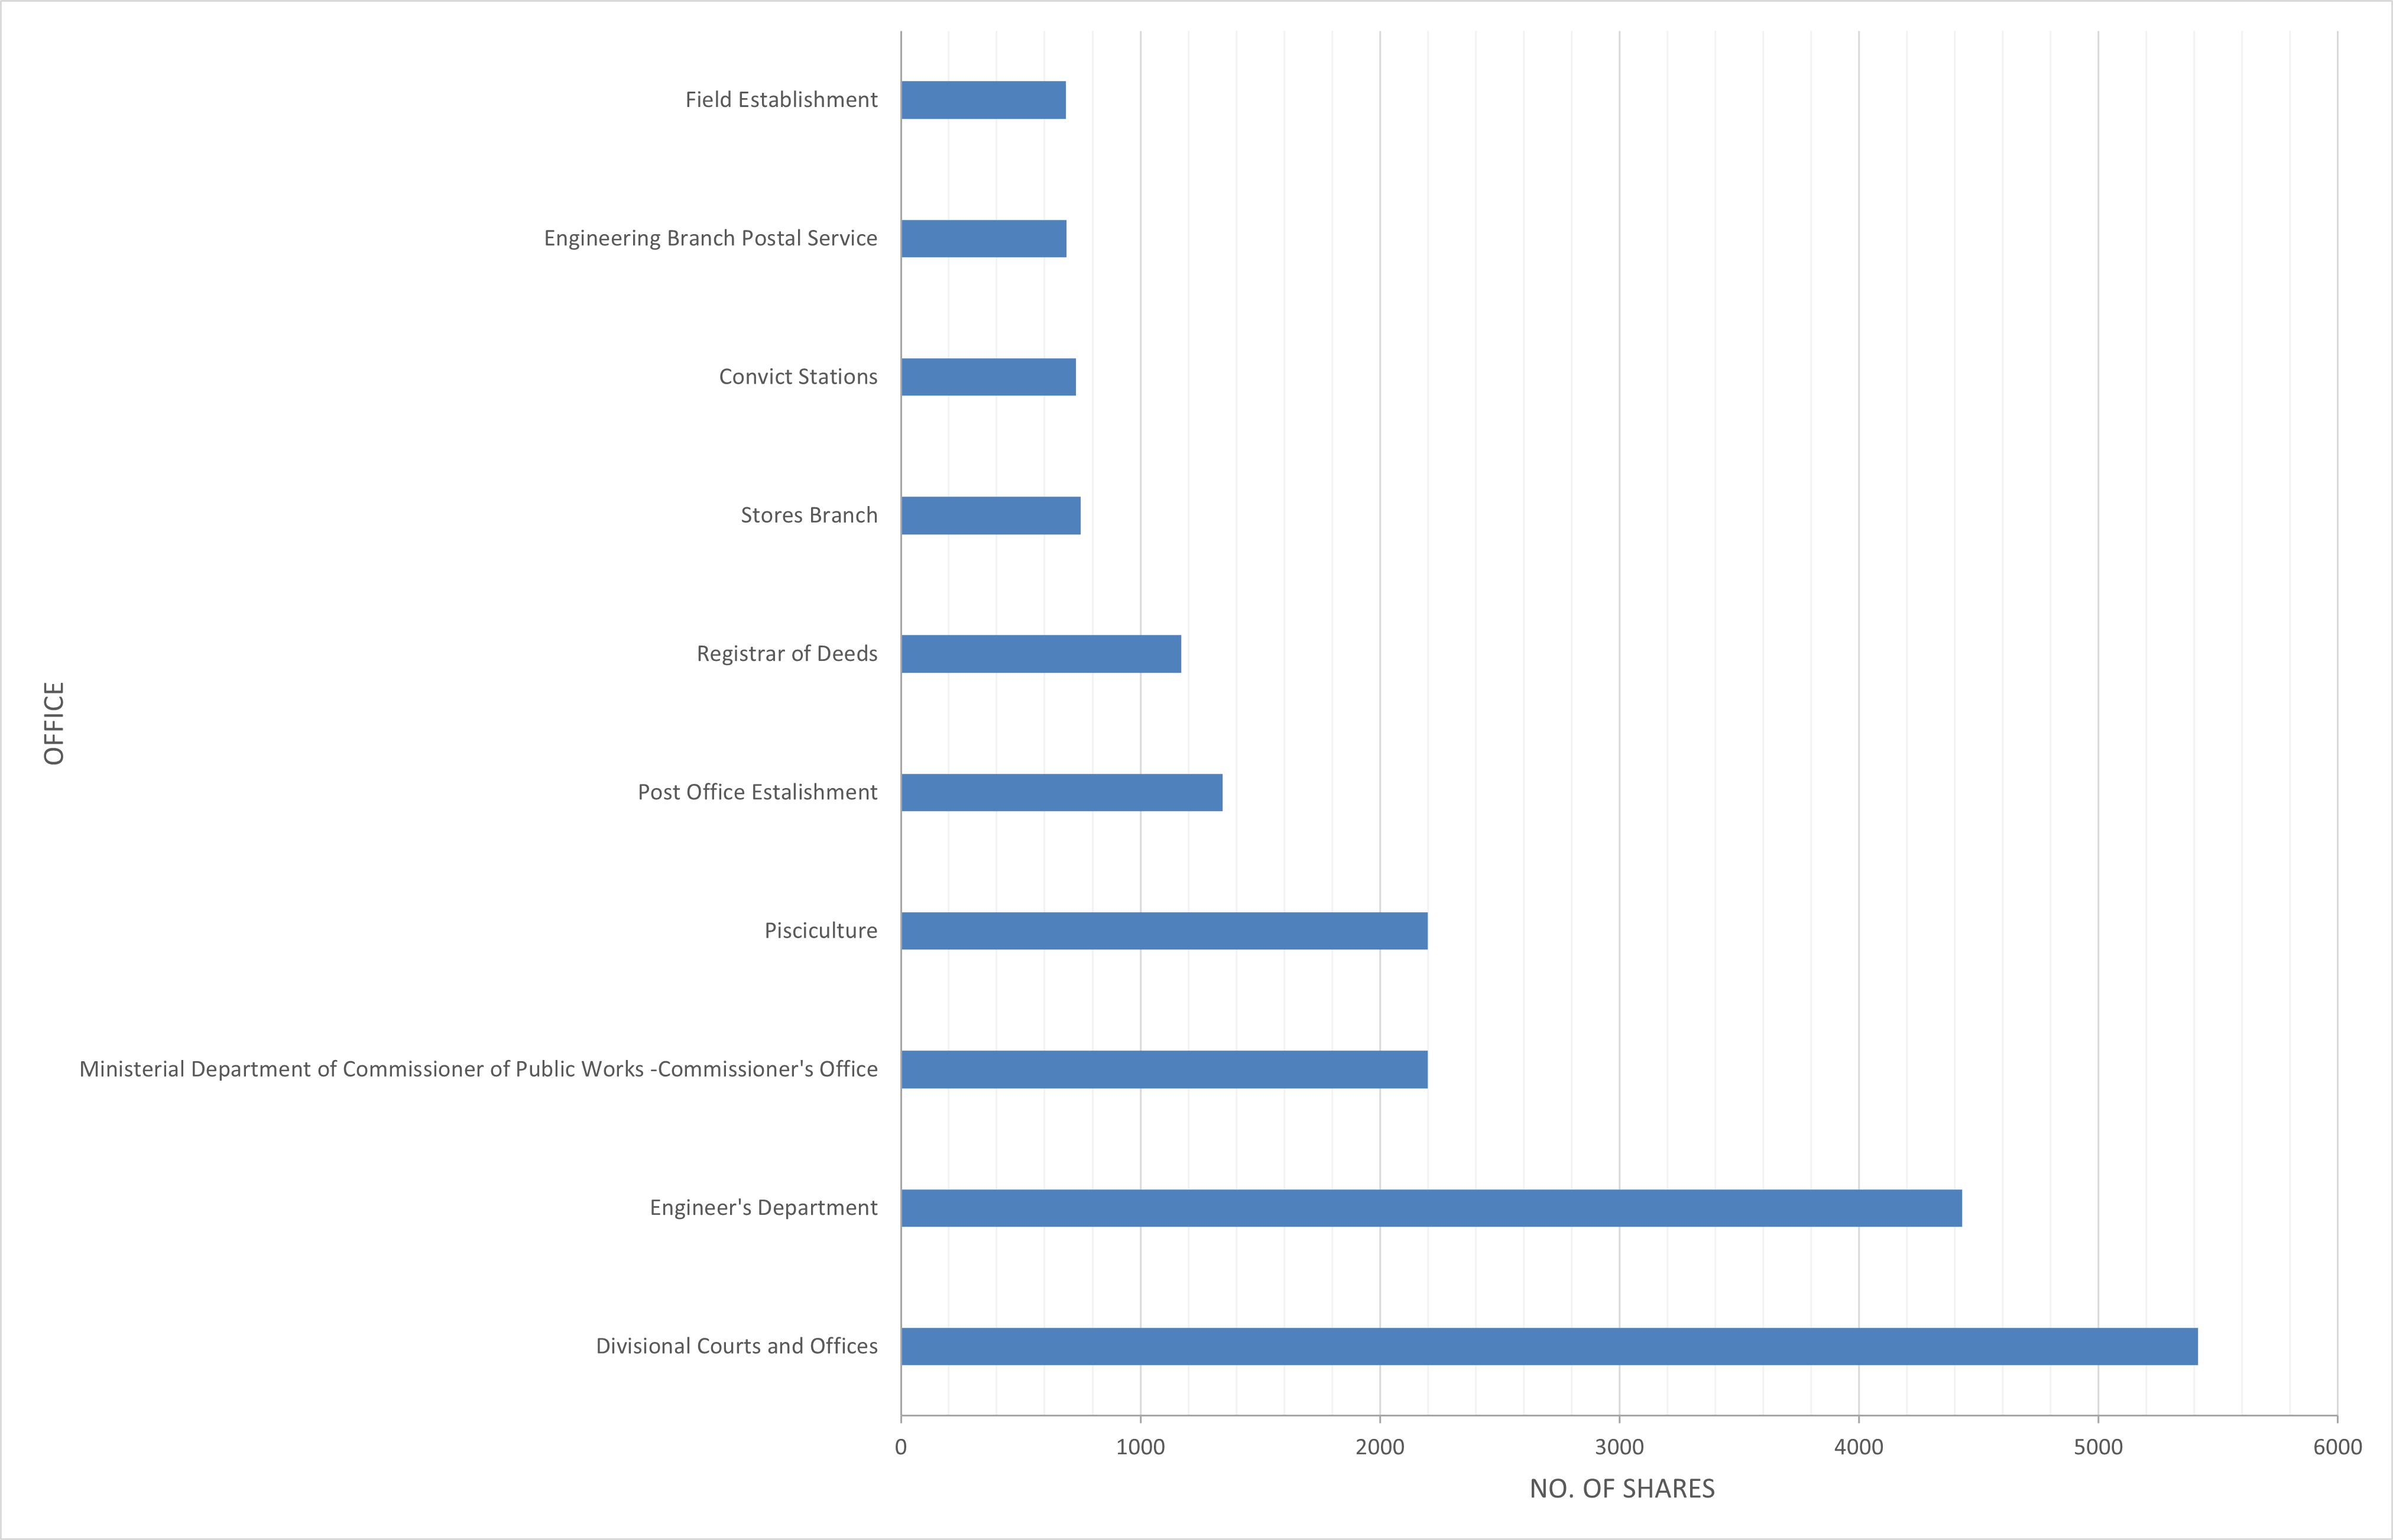
\includegraphics[width=\textwidth,height=0.5\textheight]{/Users/samanthascott/Desktop/Picture18.png}
\caption{Number of Shares per Office}
\end{figure}

According to Hunt (2005:2) as well as Transparency International (2004),
more than half of the countries' surveyed respondents perceive the
police and the judiciary as the most corrupt institutions. This
indicates that the findings found in this paper are not unique to the
Cape Colony nor to the 19th century, as there seems to be a global trend
in even more recent years. This global trend is worrying as members
working in the law enforcement and judiciary have the power to make
decisions that could impact the success of the industry, indirectly
influencing the economy.

As depicted in Figure 4.2 below, most of the corrupt civil servants
invested in real estate. As there is very little literature on the real
estate industry in the 19th century Cape Colony, there are two possible
reasons for the interest in investing in property, both linked to the
emancipation of slaves. The first hypothesis is that with the abolition
of slavery, there was an influx of `free' individuals seeking a place of
residence. The second hypothesis could be that as a result of removing a
financial asset (slaves) from the economy, a rise in inflation is
experienced. As such, the demand for property decreases as it becomes
more expensive to be in debt. With the decrease in demand, a decrease in
prices follow. This makes it more attractive to invest in property. This
attractiveness is attributed to the belief that property prices will
rise again - it is possible that civil servants may be awarded this
information before the general public.

\begin{figure}
\centering
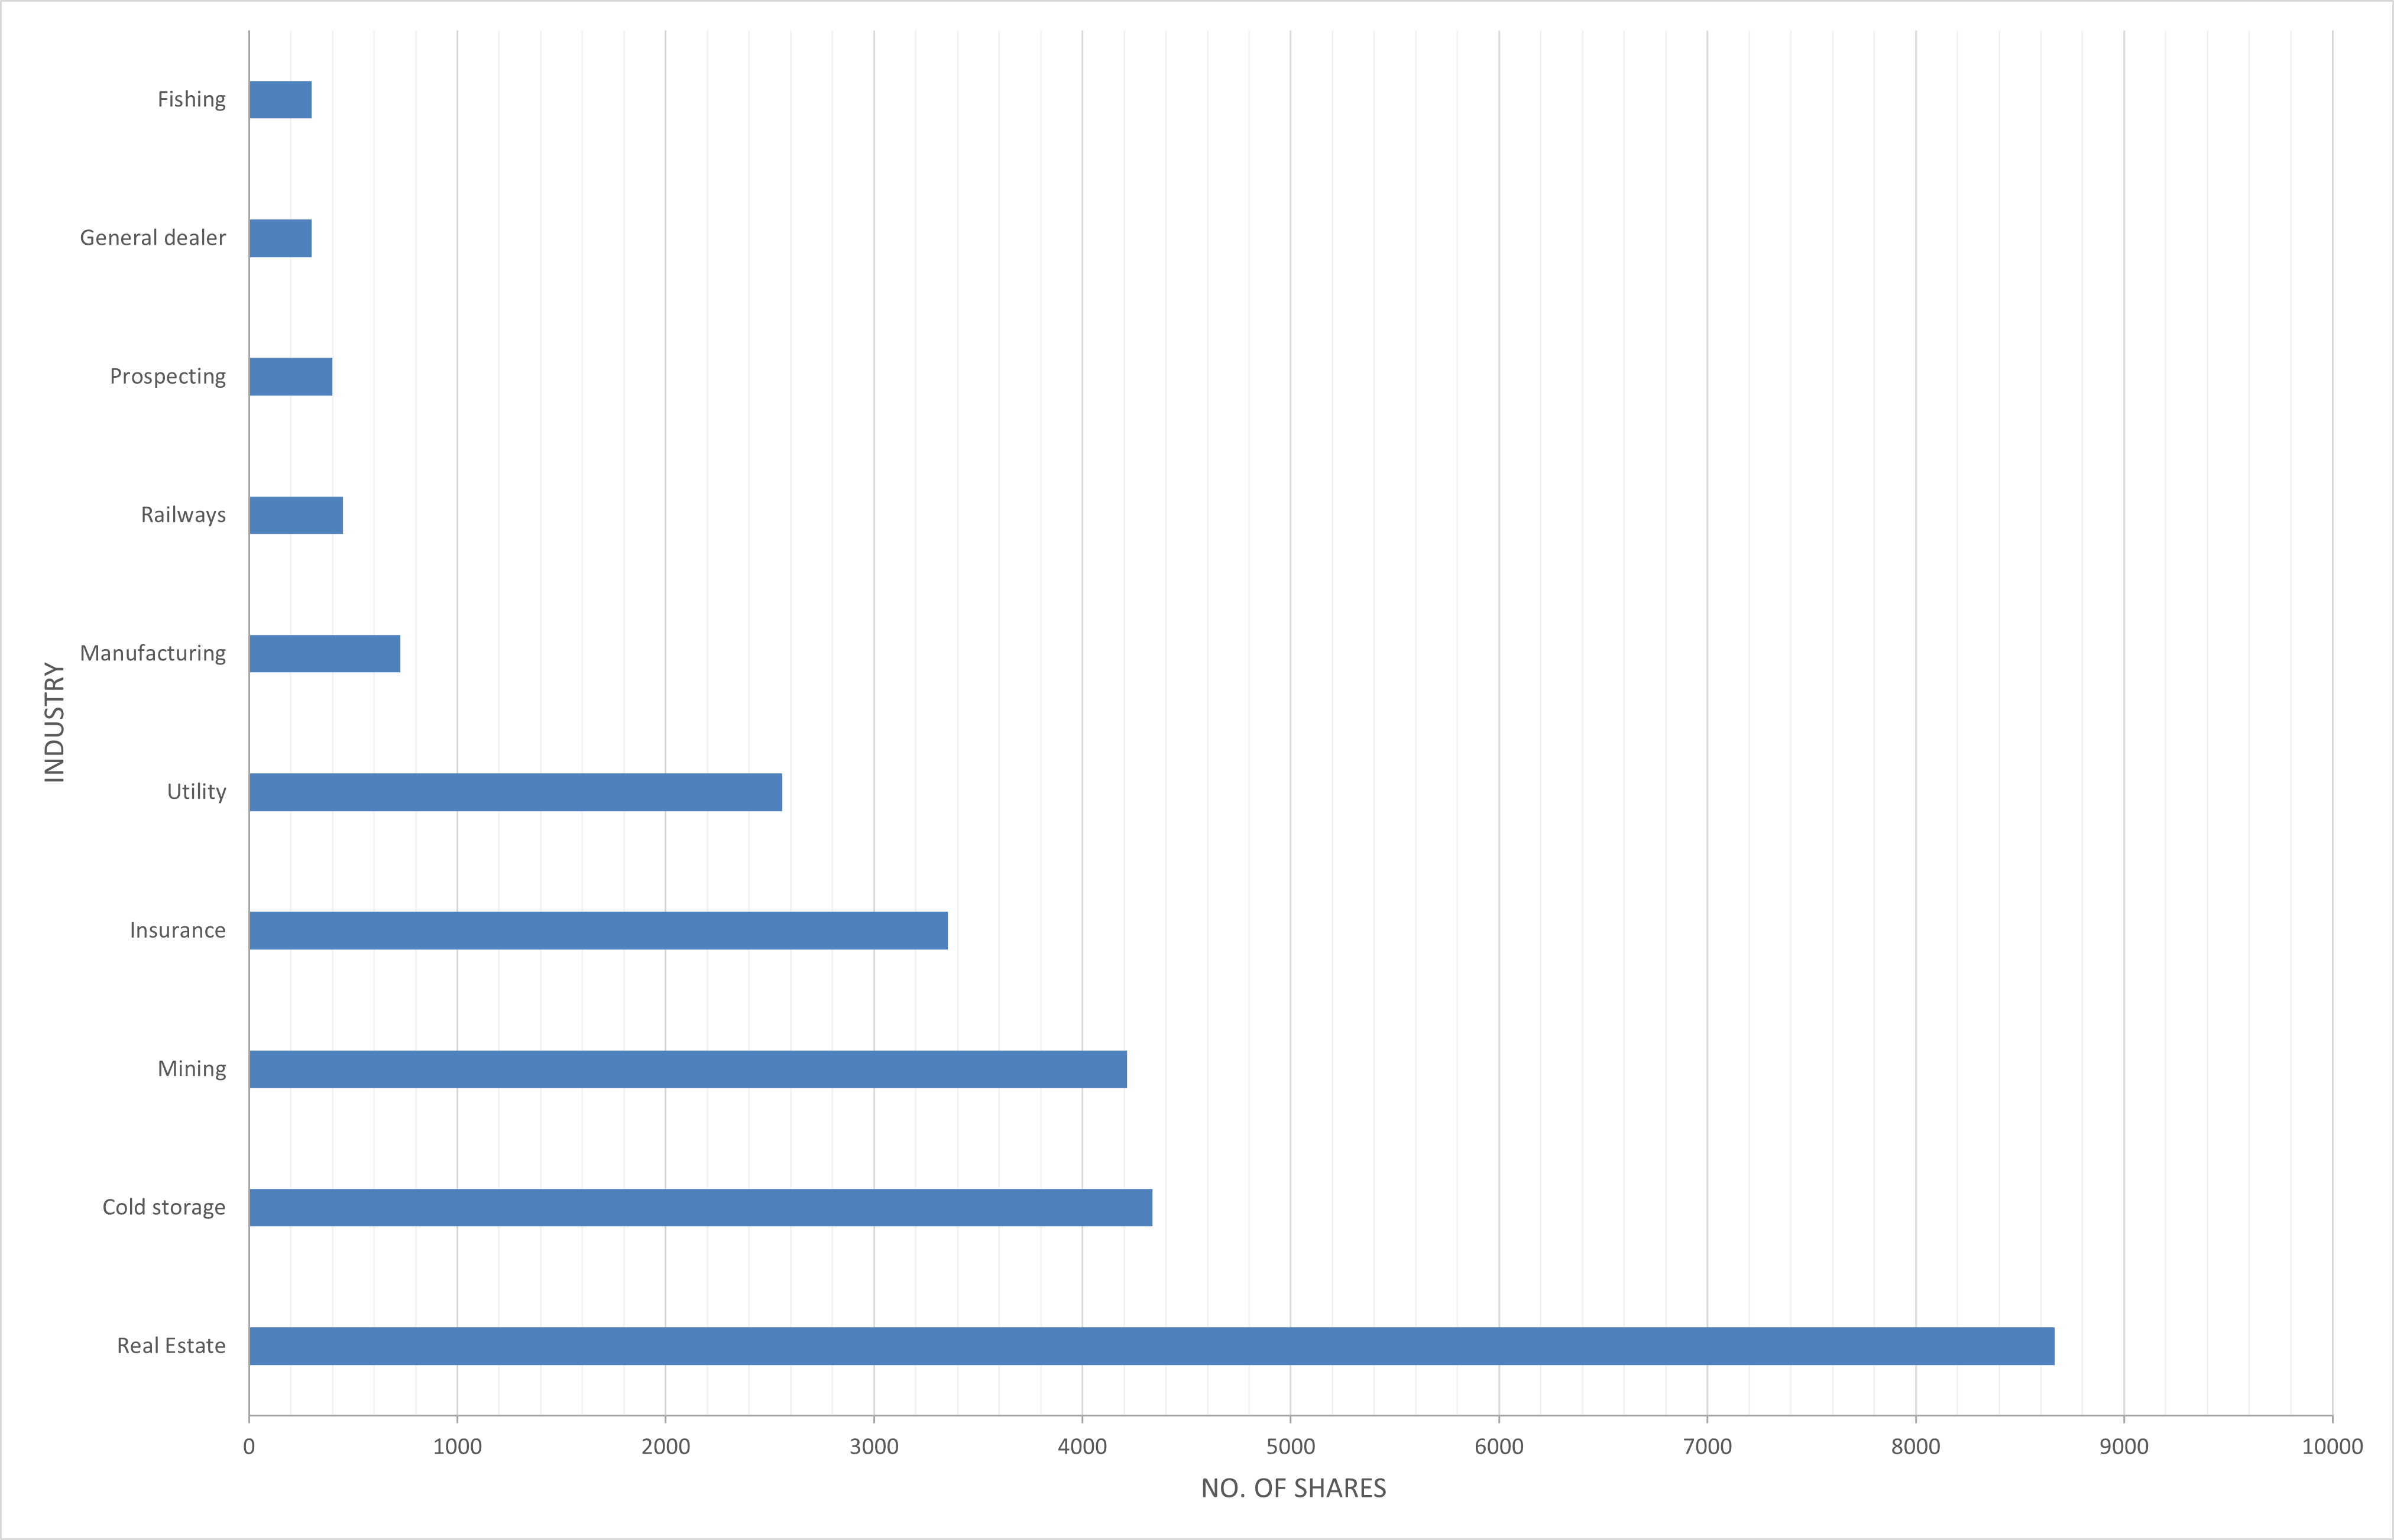
\includegraphics[width=\textwidth,height=0.5\textheight]{/Users/samanthascott/Desktop/Picture17.png}
\caption{Number of Shares per Industry}
\end{figure}

When investigating the Divisional Court and Offices corrupt employees
alone, the mining and real estate industries were invested in by the
highest number of corrupt individuals. Real estate had more shares
bought than mining. As depicted in Figure 4.3 below, 67\% of shares were
bought in the real estate industry and 29\% in the mining industry by
the corrupt employees in the Divisional Courts and Offices. The rest of
the industries make up a smaller portion. The interest in investing in
mining could be have been due to the discovery of diamonds and gold
during the mid-19th century in South Africa (Gwaindepi \& Fourie,
2020:341). The investments in the mining industry occurred after the
discovery of diamonds and gold. Further research in this field could be
done to investigate what insider information the Divisional Courts and
Offices would have had at the time that made investing in mining
attractive, apart from the discovery of diamonds and gold - which was
information known to the public. Control of other industries, for
example manufacturing of tools used in mining, that are complementary to
the mining industry could be a reason for the incentive to invest in
mining.

\begin{figure}
\centering
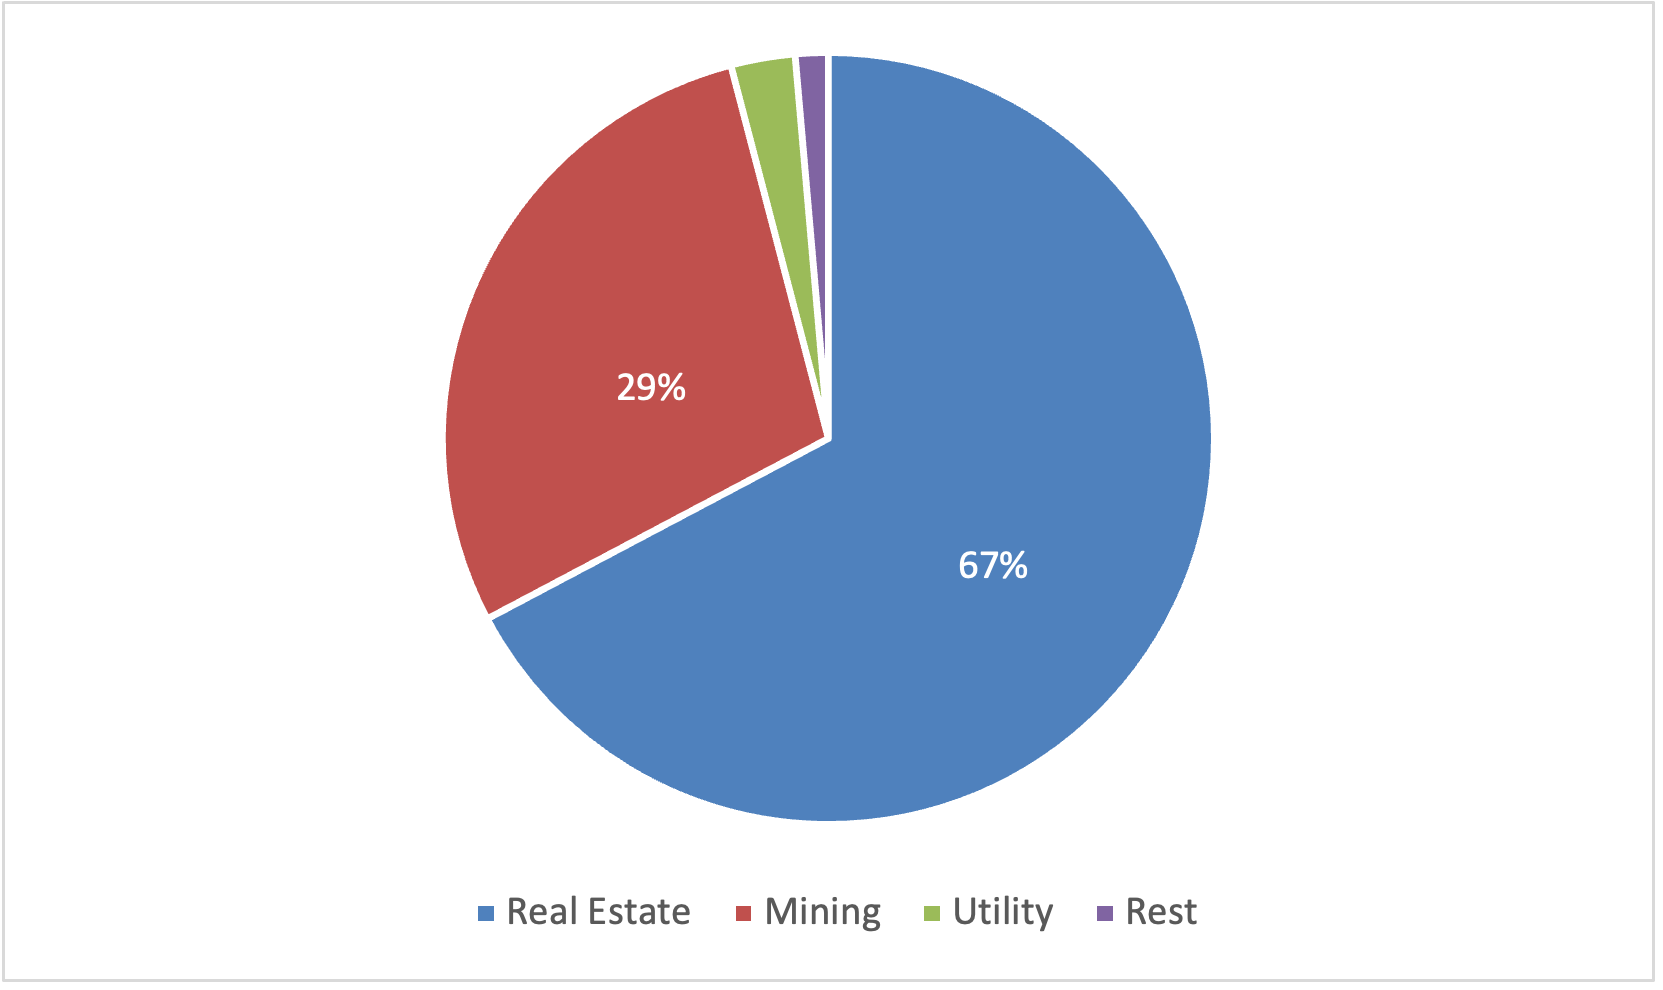
\includegraphics[width=\textwidth,height=0.45\textheight]{/Users/samanthascott/Desktop/Write_Up/Pie.png}
\caption{Number of Shares per Industry, According to Divisional Courts
and Offices}
\end{figure}

\hypertarget{limitations}{%
\section{Limitations}\label{limitations}}

This study has some limitations. The biggest issue is that the
literature and data on the topic is limited. The matched data set has
few observations, making it difficult to make informed conclusions
regarding the questions at hand. An issue with the method of matching
full names in the data sets is that the way in which first names are
written varies. For example, the list of limited liability companies
contains initials for first and second names, whereas majority of the
names in the civil servant list are written out in full. As a
consequence, when matching the names according to full name, there are
less matches than what there were in reality. When matching according to
surname alone, the issue of matching initials and full first names is
overcome. However, the likelihood of different individuals have the same
last name is high. As such, there will be more matches evident than
there would have been in reality. Another issue worth mentioning is that
more common names are more likely to produce matches, resulting in bias
results. Due to the variation in the naming of positions held in office,
it is difficult to make strong conclusions regarding the extent of power
the individuals held, without making speculative assumptions.

The act of investing and being a civil servant would only be considered
as corruption if the investment was made during the time of service. As
such, some of the matches may not be regarded as corruption as the time
of investment does not necessarily correspond with the time of active
service, creating a false representation of the individuals. Another
issue with the study is that there may have been room for human error.
There may have been physical mistakes made during the process of
entering data, as well as when compiling the two data sets. If mistakes
were made, an accurate number of corrupt individuals would not have been
found. As a result of these limitations, the number of corrupt employees
cannot be accurately predicted, and therefore the extent of corruption
cannot be commented on.

\hypertarget{conclusion}{%
\section{Conclusion}\label{conclusion}}

In conclusion, the findings suggest that corruption was present in the
19th century Cape Colony. The matching process described in methodology
presents matches between the data sets on civil servants and
shareholders of limited liability companies. The number of matches is
low in comparison to the number of observations in both data sets,
however, is still noticeable. The data sets present limitations, and the
low count of matches can be attributed to these limitations, suggesting
that the trend of corruption in civil servants may be stronger than
found. The matches indicate that most investors were in Divisional
Courts and Offices and that real estate and mining were two industries
of most interest. These findings correlate with the two key moments in
the 19th Century South Africa, namely the abolition of slavery and the
discovery of diamonds and gold. It also suggests that trace of
corruption, as found, in these industries could have had an impact on
the industries themselves and furthermore, economy of South Africa.
Thus, due to the influence civil servants could have on the decisions
regarding industries, there is an imbalance in power and information
between civil servants and the general public. It is proposed that
further research with regards to the influence of office on these
industries, particularly the Divisional Courts and Offices on real
estate is performed. It is suggested that further research on format of
the data sets used will help obtain more concise findings. Although
there are limitations endured in the matching process, the method has
resulted in a new data set through which further investigation may
occur.

\newpage

\hypertarget{reference-list}{%
\section{Reference List}\label{reference-list}}

Blackman, M. \& Dall, N. 2021. Rogues' Gallery: an Irreverent History of
Corruption in South Africa, from the VOC to the ANC. Cape Town: Penguin
Books.

Blau, B. M., Griffith, T. G. \& Whitby, R. J. 2022. On the Ethics of
``Non‑Corporate'' Insider Trading. \emph{Journal of Business Ethics},
177:79--93.

Cape of Good Hope Civil Service List, 1885-1902, CCP 11/4/1-11/4/17.
Western Cape Archives and Records Service, Cape Town.

\emph{College of Policing} {[}Online{]}. 2022. Available:
\url{https://profdev.college.police.uk/professional-profile/chief-constable/}
{[}2022, May 16{]}.

Ekama, K. \& Ross, R. 2021. The Emancipation of the Enslaved in the Cape
Colony: Historiography and Introduction. \emph{Journal of Southern
African Studies}, 47(3):405-416.

Greyling, L. \& Verhoef, G. 2017. Savings and economic growth: a
historical analysis of the Cape Colony economy, 1850--1909.
\emph{Economic History of Developing Regions}, 32(2):127-176.

Gwaindepi, A. 2018. State building in the colonial era: Public revenue,
expenditure and borrowing patterns in the Cape Colony, 1820-1910.
Unpublished doctoral dissertation. Stellenbosch: University of
Stellenbosch.

Gwaindepi, A. \& Fourie, J. 2020. Public Sector Growth in the British
Cape Colony: Evidence from New Data on Expenditure and Foreign Debt.
\emph{South African Journal of Economics}, 88(3):341-367.

Hunt, J. 2005. Why Are Some Public Officials More Corrupt Than Others?
Working Paper No.~11595. Nber, Cambridge: National Bureau of Economic
Research.

Ling, L. 2012. The ``Production'' of Corruption in China's Courts:
Judicial Politics and Decision Making in a One-Party State. \emph{Law
and Social Inquiry}, 37(4):848-877.

Maphosa, L. M. 2021. A historical analysis of joint stock companies in
the Cape Colony between 1892 and 1902. Unpublished doctoral
dissertation. Stellenbosch: University of Stellenbosch.

Myint, U. 2000. Corruption: Causes, Consequences and Cures.
\emph{Asia-Pacific Development Journal}, 7(2):33-58.

Tanzi, Vito. 1998. Corruption around the World: Causes, Consequences,
Scope, and Cures. IMF Staff Papers 45(4):559-94.

Transparency International (2004), ``Report on the Transparency
International Global Corruption Barometer 2004'',
www.transparency.org/surveys/index.html, accessed 21 May 2005.

\bibliography{Tex/ref}





\end{document}
